\documentclass[11pt]{article}
\usepackage{fullpage,url}
\usepackage{amsmath,amsthm,amssymb}
\usepackage{graphicx}
\usepackage{eso-pic}
\usepackage{bm}
\usepackage{caption}
\usepackage{picins}   
\usepackage{microtype}
\usepackage{subcaption}
\usepackage{url}
\usepackage{enumerate}
\usepackage{pdfpages}
\usepackage{hyperref}
\usepackage[letterpaper,top=1in,bottom=1in,left=1in,right=1in,nohead]{geometry}

\newcommand{\PhiB}{\mathbf{\Phi}}
\newcommand{\Ll}{\mathcal{L}}
\newcommand{\Nn}{\mathcal{N}}
\newcommand{\Uu}{\mathcal{U}}
\newcommand{\Ee}{\mathcal{E}}
\newcommand{\Aa}{\mathcal{A}}
\newcommand{\Hh}{\mathcal{H}}
\newcommand{\Ii}{\mathcal{I}}
\newcommand{\Vv}{\mathcal{V}}
\newcommand{\Ff}{\mathcal{F}}
\newcommand{\Dd}{\mathcal{D}}
\newcommand{\Tt}{\mathcal{T}}
\newcommand{\Pp}{\mathcal{P}}
\newcommand{\Ss}{\mathcal{S}}
\newcommand{\Cc}{\mathcal{C}}
\newcommand{\Oo}{\mathcal{O}}
\newcommand{\Bb}{\mathcal{B}}
\newcommand{\Rr}{\mathcal{R}}
\newcommand{\Rm}{\mathrm{R}}
\newcommand{\CB}{\mathbf{C}}
\newcommand{\RB}{\mathbf{R}}
\newcommand{\xB}{\mathbf{x}}
\newcommand{\yB}{\mathbf{y}}
\newcommand{\XB}{\mathbf{X}}
\newcommand{\YB}{\mathbf{Y}}
\newcommand{\fB}{\mathbf{f}}
\newcommand{\tB}{\mathbf{t}}
\newcommand{\ZB}{\mathbf{Z}}
\newcommand{\SB}{\mathbf{S}}
\newcommand{\GB}{\mathbf{G}}
\newcommand{\AB}{\mathbf{A}}
\newcommand{\WB}{\mathbf{W}}
\newcommand{\TB}{\mathbf{T}}
\newcommand{\IB}{\mathbf{I}}

\newcommand{\omitme}[1]{}
\newtheorem*{lemma}{Lemma}
\newtheorem{case}{Case}

\makeatletter
\newcommand{\specialnumber}[1]{%
  \def\tagform@##1{\maketag@@@{(\ignorespaces##1\unskip\@@italiccorr#1)}}%
}

\setlength{\parindent}{0in}
\setlength{\parskip}{6pt}

\DeclareMathOperator{\E}{E}
\DeclareMathOperator{\Var}{Var}
\DeclareMathOperator{\Unif}{Unif}

\begin{document}
\thispagestyle{empty}
{\large{\bf CS6320: 3D Computer Vision \hfill Prateep Mukherjee(u0876583)}}\\

{\LARGE{\bf Homework 3}}
\vspace{0.2\baselineskip}
\hrule


  \vspace{-10pt}
\section{Theoretical Problems}
    \vspace{-10pt}
    
 \subsection{}   
\textbf{(a)} 

\begin{figure*}[!hbt]
\centering
\begin{tabular}{cc  cc}
  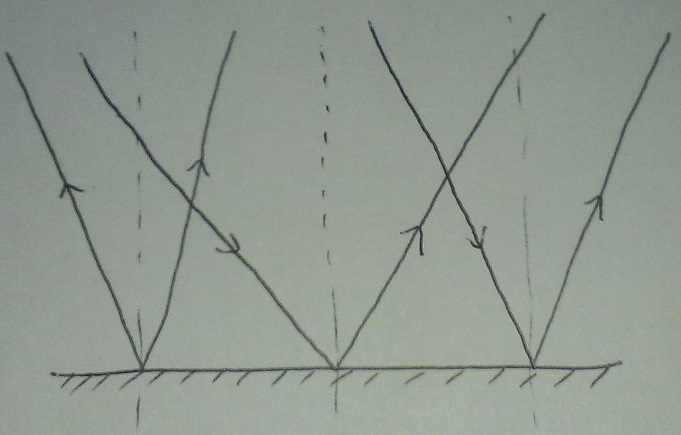
\includegraphics[width=0.5\textwidth]{IMAG0252.jpg} &
  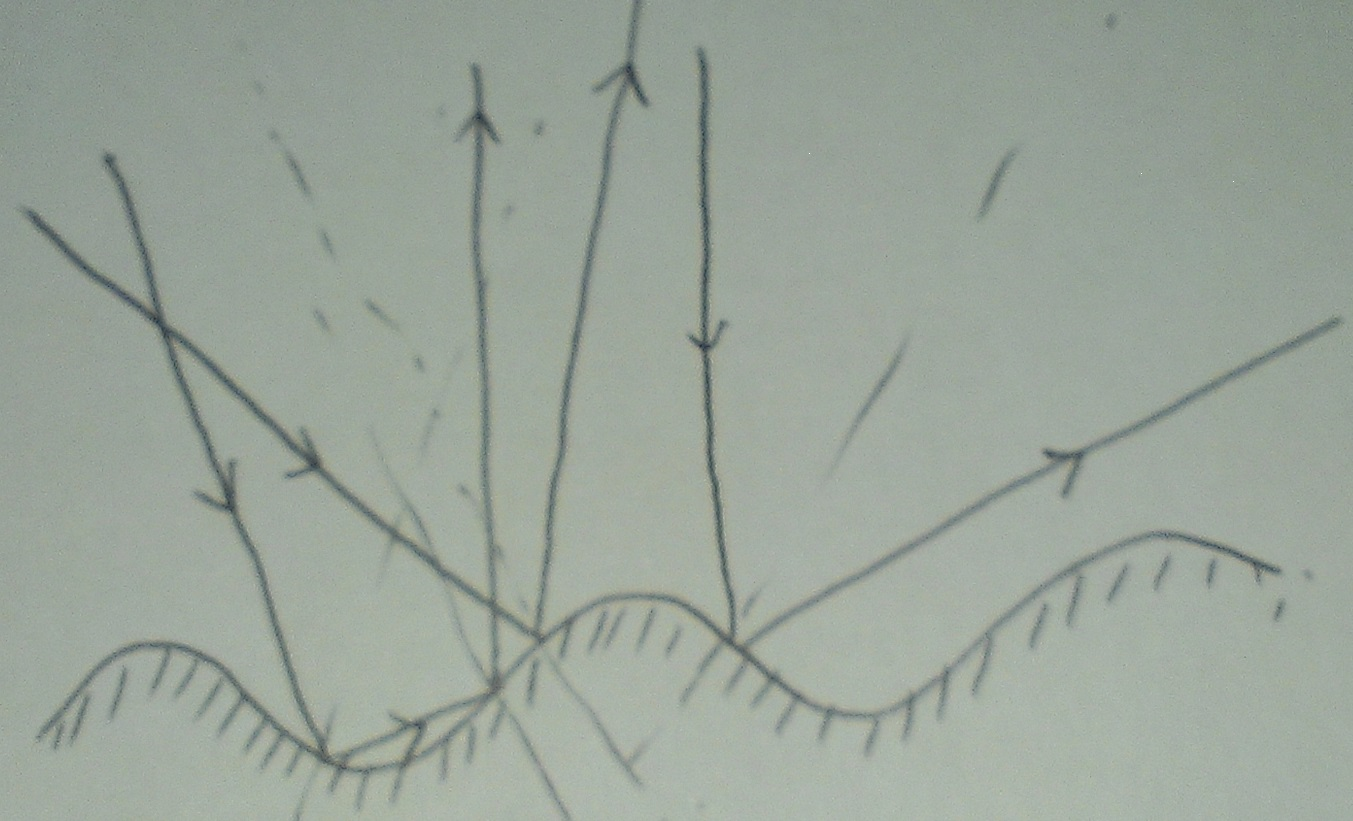
\includegraphics[width=0.53\textwidth]{IMAG0253.jpg} \\
  (a) & (b) 
 \end{tabular}
 \vspace{-10pt}
 \caption{(a) \textbf{Specular reflection} on a smooth even surface; \textbf{Diffuse reflection} on an uneven surface.}
 \label{fig1}
\end{figure*}

Fig. \ref{fig1} shows the scenarios for specular and diffuse reflection. For \textbf{specular  reflection}, all of the light rays are reflected along same direction. For \textbf{diffuse reflection}, the direction of light rays is random and also reflect from the uneven surface. Since the concentration of light intensity is greater for specular reflection, the spot on the surface where it reflects from looks brighter.

\begin{figure*}[!hbt]
\centering
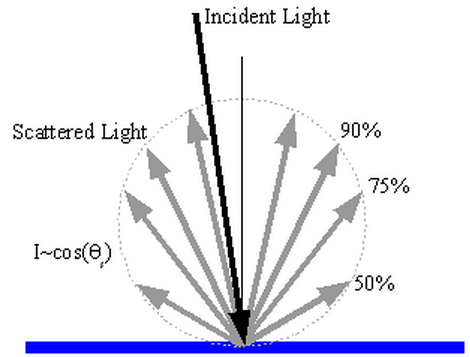
\includegraphics[width=0.5\textwidth]{pic3.png}
\vspace{-10pt}
\caption{Lambertian, or diffuse, scatter of light is governed by a cosine intensity relationship}
\label{fig2}
\end{figure*}

\par \textbf{(b)}  For Lambertian surfaces, the directional hemispheric reflectance is independent of illumination direction. A formal model is given by \emph{bidirectional reflectance distribution function}, or \textbf{BRDF} is independent of outgoing direction. Therefore, the radiance($\rho$) is independent of viewing angle. Fig. \ref{fig2} shows an example of this. 

\subsection{}
\textbf{(a)} As derived in class, the radiosity($B(x,y)$) can be written in terms of albedo($\rho$) and the angles($\theta_e, \theta_i$) as:
\vspace{-10pt}
\begin{align}
  B(x,y) =&  \rho \frac{\cos \theta_e}{\cos \theta_i} \\
       =&  \rho \frac{<\widehat{N_L}, \widehat{N}>}{<\widehat{N_l}, \hat{N} >}
 \label{eq4}
\end{align}

where, $\widehat{N_L}$ denotes the normalized normal of light source direction, $\widehat{N_l}$ denotes normalized normal of the lens direction and $\widehat{N}$ denotes the surface normal at $(x,y)$. Assuming viewer centered geometry, eq. \ref{eq4} reduces to :
\vspace{-10pt}
\begin{align}
B(x,y)  =& \rho \frac{ < \widehat{(-p_L, -q_L, 1)}, \widehat{(-p,-q,1)}> }{ < \widehat{(-p_l,-q_l,1)}, \widehat{(-p,-q,1)} > } \notag \\
\implies B(x,y) =& \rho \cdot \frac{p_L p+q_L q + 1}{ p_l p + q_l q + 1} \sqrt{ \frac{p_L^2 + q_L^2 + 1}{p_l^2 + q_l^2 + 1} } 
\label{eq5}
\end{align}
\vspace{-10pt}
Eq. \ref{eq5} shows the reflectance map $R(p,q)$.

\textbf{(b)} To generate isodensity curves of constant brightness in $R(p,q)$, we set $B(x,y) = c$, where $c$ is a constant. This reduces eq. \ref{eq5} to:
\vspace{-10pt}
\begin{equation}
 c_1 \cdot (1+p_l p + q_lq) = c_2 \cdot (1+p_L p + q_L q) 
 \label{eq6}
\end{equation}

where $c_1 = c \cdot \sqrt{p_l^2 + q_l^2 + 1}$ and $c_2 = \rho \cdot \sqrt{p_L^2 + q_L^2 + 1}$. Eq. \ref{eq4} shows that the isodensity curves of constant brightness are lines. 

\textbf{(c)} The contours of constant brightness of an image of sphere are straight lines in the $(p,q)$ frame.

\textbf{(d)} Fig. \ref{fig4} shows the isocontours from multiple images. 

\begin{figure*}[!hbt]
\centering
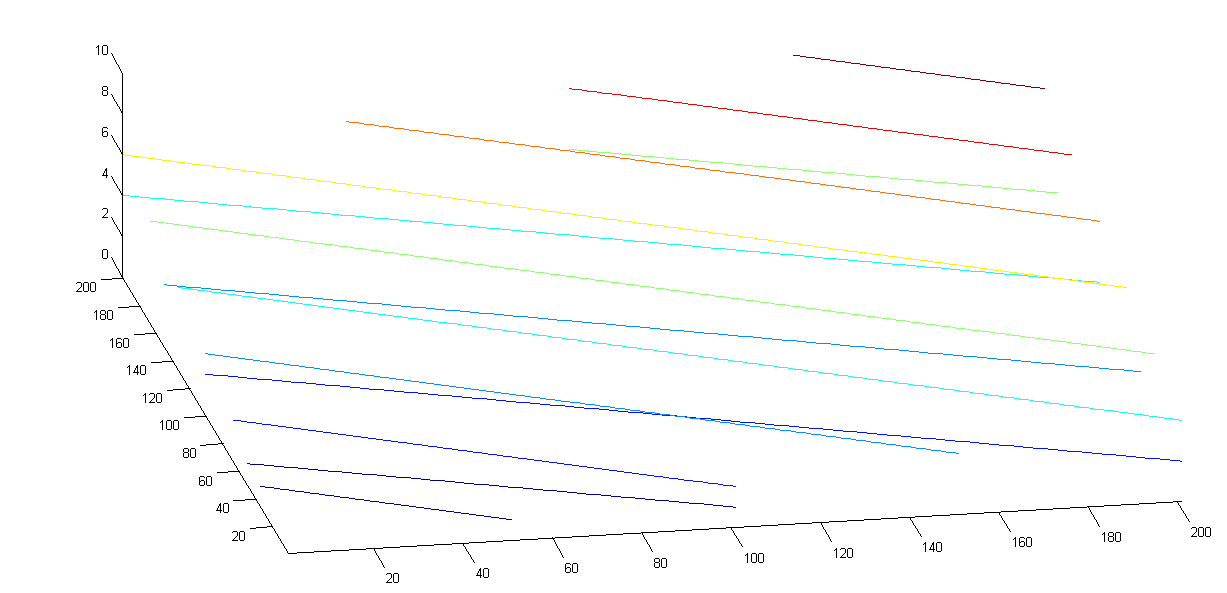
\includegraphics[width=0.5\textwidth]{q2d.png}
\caption{Lines from two different images}
\label{fig4}
\end{figure*}
\vspace{-10pt}
\subsection{} 
\textbf{a)} Given $Z = -\frac{Bf}{d}$, we can write the 1st derivative as $\frac{\partial Z}{\partial d} = \frac{Bf}{d^2}$. Change in depth($\triangle Z$) with disparity($\triangle d$) can be approximated as : $\frac{\partial Z}{\partial d} = \lim\limits_{\triangle d \rightarrow 0}\frac{\triangle Z}{\triangle d} $, which says that  $\frac{\partial Z}{\partial d}$ approximates to $\frac{\triangle Z}{\triangle d}$ under $\lim\limits_{\triangle d \rightarrow 0}$. Fig. \ref{fig3} shows the plot of the function $\frac{\partial Z}{\partial d}$. As seen change in depth decreases with change in disparity. 
\vspace{-10pt}
\begin{figure*}[[!hbt]
\centering
  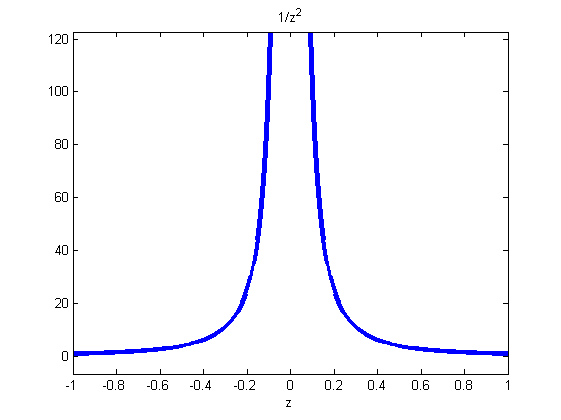
\includegraphics[width=0.5\textwidth]{pic4.png}
  \caption{Plot of $\frac{\partial Z}{\partial d}$ vs $d$.}
%  \vspace{-10pt}
  \label{fig3}
\end{figure*}

\textbf{b)} The partial derivatives of $Z$ wrt $B,f$ and $d$ look like:
\vspace{-10pt}
\begin{equation}
\frac{\partial Z}{\partial d} = \frac{Bf}{d^2},  \; \; \frac{\partial Z}{\partial B} = -\frac{f}{d}, \; \; \frac{\partial Z}{\partial f} = -\frac{B}{d} 
\label{eq1}
\end{equation}

Plugging terms in eq. \ref{eq1} into the error estimate for $Z$, we get:
\vspace{-5pt}
\begin{equation}
\delta Z = \sqrt{ (\frac{Bf}{d^2} \delta d)^2 + (\frac{f}{d} \delta B)^2 + (\frac{B}{d} \delta f)^2}
\label{eq2}
\end{equation}
\vspace{-5pt}
Eq. \ref{eq2} shows that $\delta Z$ has a linear relation with baseline width($B$) and focal length($f$).

\textbf{(c)} We can compute the relative error $\delta Z$ as follows:
\vspace{-10pt}
\begin{align}
\frac{\delta Z}{Z} =& -\frac{d}{Bf}  \sqrt{ (\frac{Bf}{d^2} \delta d)^2 + (\frac{f}{d} \delta B)^2 + (\frac{B}{d} \delta f)^2} \notag \\
=& -\sqrt{ (\frac{\delta d}{d})^2 + (\frac{\delta Z}{Z})^2  + (\frac{\delta f}{f})^2 } \notag \\
\implies \| \frac{\delta Z}{Z} \| =&  \sqrt{ (\frac{\delta d}{d})^2 + (\frac{\delta Z}{Z})^2  + (\frac{\delta f}{f})^2 } 
\label{eq3}
\end{align}

From eq. \ref{eq3}, if we want measure accuracy of features we assume $\delta B = 0$ and $\delta f = 0$. This gives us $\frac{\delta Z}{Z} = \frac{\delta d}{d} $. So, the features should be measured with same accuracy as depth map in order to get a relative error $< 1\%$.

\vspace{-10pt}
\section{Practical Problems}
 \vspace{-10pt}
 
 The problem of generating shape from shading is solved in two stages. First, we have to generate the albedo map and the normals to the surface. Next, we generate a depth map from the above normals. I describe the approach to both these in order.
 
 \subsection{Generating Normals}
 \vspace{-10pt}
 For lambertian surfaces, intensity at any point on a surface is given as:
  \vspace{-10pt}
 \begin{equation}
    I = \rho \cdot <\hat{N},\hat{ N_L} >
    \label{eq7}
 \end{equation}
 where $\hat{N}$ is the normalized normal at the surface point, $\hat{N_L}$ is the reflected light direction normalized. 	In order to determine $\hat{N}$, we use multiple($\ge3$) light sources which are not in the same plane. Thus, eq. \ref{eq7} can be written for multiple light sources as follows:
 \vspace{-10pt}
 \begin{align*}
  I_1 =& \rho \cdot ( N_x \cdot L_{1x} + N_y \cdot L_{1y} + N_z \cdot L_{1z}) \\
  I_2 =& \rho \cdot ( N_x \cdot L_{2x} + N_y \cdot L_{2y} + N_z \cdot L_{2z}) \\
  I_3 =& \rho \cdot ( N_x \cdot L_{3x} + N_y \cdot L_{3y} + N_z \cdot L_{3z}) \\
     &  \vdots \\
  I_n =& \rho \cdot ( N_x \cdot L_{nx} + N_y \cdot L_{ny} + N_z \cdot L_{nz}) 
 \end{align*}

We fold the normal($N$) and the albedo($\rho$) into one vector (\textbf{G}). Assume $\mathbf{\Vv}$ denotes a vector of light source directions.
\vspace{-10pt}
\begin{align*}
\mathbf{\Vv} = \begin{pmatrix} 
  L_1^{T} \\
  L_2^{T} \\
  \cdots \\
  L_n^{T} \\
\end{pmatrix}
\end{align*}

For $n > 3$, we can solve the equations with least squares as follows:

\begin{align*}
  \Vv \GB =& \IB \\
 \implies  \Vv \Vv^{T} \GB =& \Vv^{T} \IB \\
 \implies \GB =&  (\Vv \Vv^{T})^{-1} \Vv^{T} \IB \\
\end{align*}

Therefore, the albedo($\rho(x,y)$) and the normals to the surface($N$) can be written as:

\begin{align}
\rho(x,y) &= \| \GB\| \label{eq8} \\
N(x,y)  &= \GB / {\rho(x,y)} \label{eq9} 
\end{align}

\clearpage
\subsection{Generating Depth Map}
 
 \begin{figure*}[!hbt]
 \centering
 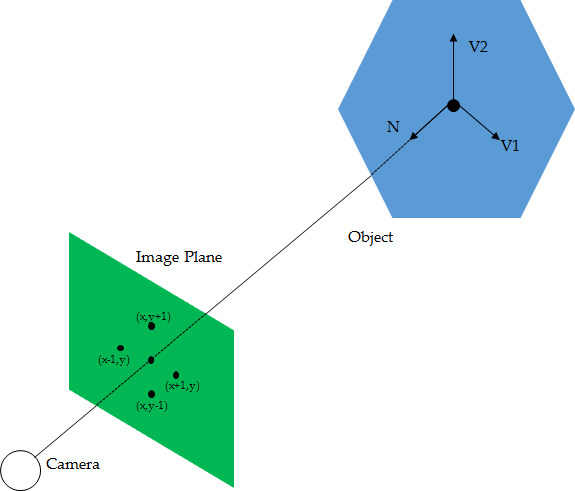
\includegraphics[width = 0.5\textwidth]{pic5.png}
 \caption{Schematic diagram showing the normals for the image plane, camera and 3D world object. }
 \label{fig4}
 \end{figure*}
 
 From Fig. \ref{fig4}, the normal at surface($N$) must be orthogonal to $V1$ which gives:
 \vspace{-10pt} 
 \begin{eqnarray}
   V1 &=& (x+1,y,z_{(x+1,y)}) - (x,y,z_{(x,y)}) \notag \\ 
        &=& (1,0, z_{(x+1,y)} - z_{(x,y)}) \notag \\
\implies N \cdot V1 &=& 0 \notag \\
\implies (N_x, N_y, N_z) \cdot (1, 0, z_{(x+1,y)} - z_{(x,y)}) &=& 0 \notag \\
\implies N_x + N_z(z_{(x+1,y)} - z_{(x,y)}) &=& 0
\label{eq10}
 \end{eqnarray}

 Again, the normal at surface($N$) must be perpendicular to $V2$ which gives:
 \vspace{-10pt}
 \begin{eqnarray}
  V2 &=& (x,y+1,z_{(x,y+1)}) - (x,y,z_{(x,y)}) \notag \\ 
     &=& (0,1, z_{(x,y+1)} - z_{(x,y)}) \notag \\
\implies N \cdot V2 &=& 0 \notag \\
\implies (N_x, N_y, N_z) \cdot (0, 1, z_{(x,y+1)} - z_{(x,y)}) &=& 0 \notag \\
\implies N_y + N_z(z_{(x,y+1)} - z_{(x,y)}) &=& 0
\label{eq11} 
 \end{eqnarray}
 
 \vspace{-10pt}
 Taking boundary conditions at pixels where $N$-values are not available, we take the forward direction for depth calculation, which gives:
  \vspace{-10pt}
 \begin{align}
  -N_x + N_z(z_{(x-1,y)} - z_{(x,y)}) &= 0 \label{eq12} \\
  -N_y + N_z(z_{(x,y-1)} - z_{(x,y)}) &= 0 \label{eq13} 
  \vspace{-10pt}
 \end{align}
 
 Putting together Eqs. (\ref{eq10}, \ref{eq11}, \ref{eq12}, \ref{eq13}) into a sparse matrix($M$), we can get the following system of equations:
 \vspace{-5pt}
 \begin{equation}
   M \cdot z = v 
   \label{eq14}
 \end{equation}

Here $M \in \Re^{2*S,S}$, where $S$ is the size of the image, $z$ is a vector($|z| = S$) of pixels of the image, and $v$ is a vector of length $2*S$ of x and y components of normals($N_x, N_y$) repeated for every pixel. It is easily seen that $M$ is a sparse matrix. To speed up our computation, I use only those pixels in the image which had moderately high intensity. These pixels are labeled together in a binary image, \textbf{mask}.

In order to solve Eq. \ref{eq14}, we invert matrix $M$ using QR decompositon and solve for $z$.  Figures (\ref{fig4},\ref{fig5},\ref{fig6}) shows the results for synthetic-image, dog and sphere images respectively.

\begin{figure}[!hbt]
\centering
  \vspace{-5pt}
  \begin{subfigure}[h]{0.3\textwidth}
    \centering
    
\includegraphics[width = \textwidth]{../synth-images/im1.png}
  \end{subfigure} 
    \begin{subfigure}[h]{0.3\textwidth}
    \centering
    
\includegraphics[width = \textwidth]{../synth-images/im2.png}
  \end{subfigure} 
    \begin{subfigure}[h]{0.3\textwidth}
    \centering
    
\includegraphics[width = \textwidth]{../synth-images/im3.png}
  \end{subfigure} 
  
  
    \begin{subfigure}[h]{0.3\textwidth}
    \centering
    
\includegraphics[width = \textwidth]{../synth-images/im4.png}
  \end{subfigure} 
   \begin{subfigure}[h]{0.3\textwidth}
    \centering
    
\includegraphics[width = \textwidth]{../synth-images/mask.png}
  \end{subfigure} 
   \begin{subfigure}[h]{0.3\textwidth}
    \centering
    \includegraphics[width = \textwidth]{../synth-images/normals.png}
  \end{subfigure}
  
  \begin{subfigure}[h]{0.3\textwidth}
    \centering
    
\includegraphics[width = \textwidth]{../synth-images/albedo.png}
  \end{subfigure} 
  \begin{subfigure}[h]{0.02\linewidth}
    \centering
    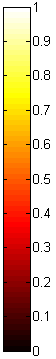
\includegraphics[width = 7mm, height = 48mm]{../synth-images/colorbar.png}
  \end{subfigure} 
    \begin{subfigure}[h]{0.5\textwidth}
    \centering
    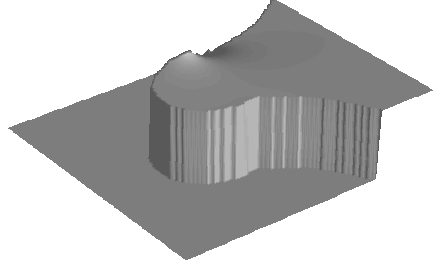
\includegraphics[width = \textwidth]{../synth-images/depthMap.png}
  \end{subfigure} 
   
  \caption{\textbf{Synth-images} dataset. Images shown in order are 4 original images, mask image, \emph{quiver-plot} of surface normals, albedo map and the reconstructed depth.}
  \label{fig4}
  \end{figure}

\begin{figure}[!hbt]
\centering
  \vspace{-5pt}
  \begin{subfigure}[h]{0.3\textwidth}
    \centering
    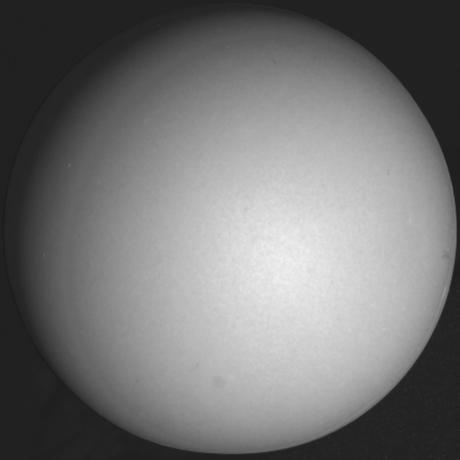
\includegraphics[width = \textwidth]{../sphere-images/real1.jpg}
  \end{subfigure} 
    \begin{subfigure}[h]{0.3\textwidth}
    \centering
    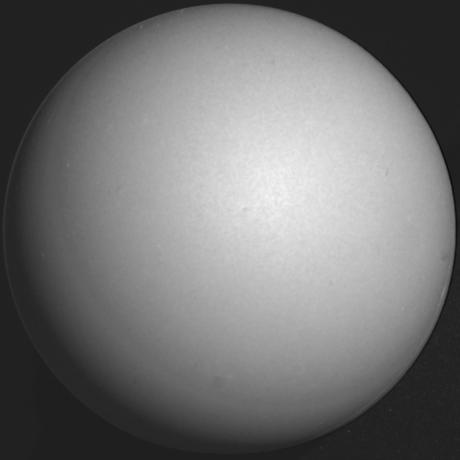
\includegraphics[width = \textwidth]{../sphere-images/real2.jpg}
  \end{subfigure} 
    \begin{subfigure}[h]{0.3\textwidth}
    \centering
    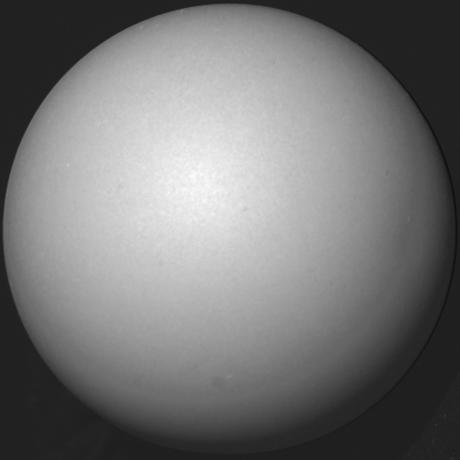
\includegraphics[width = \textwidth]{../sphere-images/real3.jpg}
  \end{subfigure} 
  
  
    \begin{subfigure}[h]{0.3\textwidth}
    \centering
    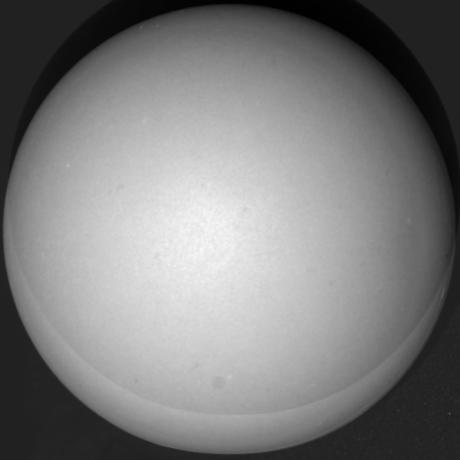
\includegraphics[width = \textwidth]{../sphere-images/real4.jpg}
  \end{subfigure} 
   \begin{subfigure}[h]{0.3\textwidth}
    \centering
    
\includegraphics[width = \textwidth]{../sphere-images/mask.png}
  \end{subfigure} 
%   \begin{subfigure}[h]{0.3\textwidth}
%    \centering
%    \includegraphics[width = \textwidth]{../sphere-images/normals.png}
%  \end{subfigure}
  
  \begin{subfigure}[h]{0.3\textwidth}
    \centering
    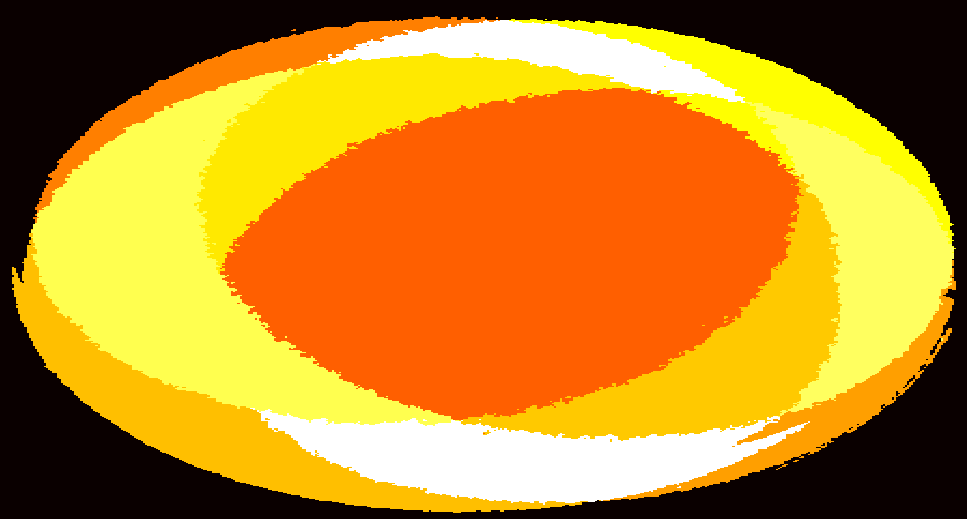
\includegraphics[width = \textwidth]{../sphere-images/albedo.png}
  \end{subfigure} 
  \begin{subfigure}[h]{0.02\linewidth}
    \centering
    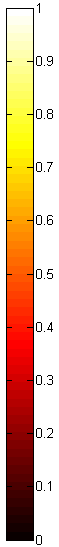
\includegraphics[width = 7mm, height = 48mm]{../sphere-images/colorbar.png}
  \end{subfigure} 
    \begin{subfigure}[h]{0.5\textwidth}
    \centering
    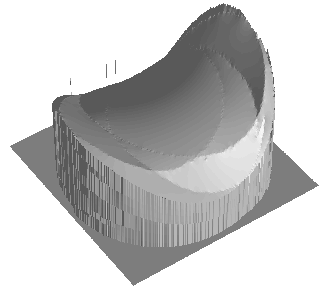
\includegraphics[width = \textwidth]{../sphere-images/depthMap.png}
  \end{subfigure} 
   
  \caption{\textbf{Sphere-images} dataset. Images shown in order are 4 original images, mask image, \emph{quiver-plot} of surface normals, albedo map and the reconstructed depth.}
  \label{fig5}
  \end{figure}

\begin{figure}[!hbt]
\centering
  \vspace{-5pt}
  \begin{subfigure}[h]{0.3\textwidth}
    \centering
    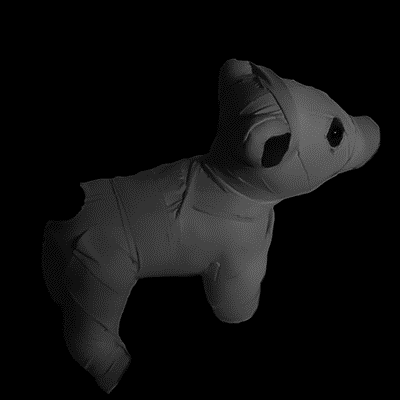
\includegraphics[width = \textwidth]{../dog-png/dog1.png}
  \end{subfigure} 
    \begin{subfigure}[h]{0.3\textwidth}
    \centering
    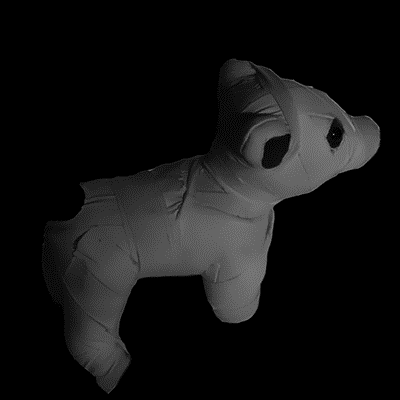
\includegraphics[width = \textwidth]{../dog-png/dog2.png}
  \end{subfigure} 
    \begin{subfigure}[h]{0.3\textwidth}
    \centering
    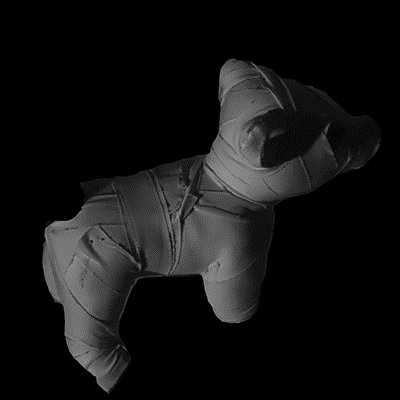
\includegraphics[width = \textwidth]{../dog-png/dog3.png}
  \end{subfigure} 
  
  
    \begin{subfigure}[h]{0.3\textwidth}
    \centering
    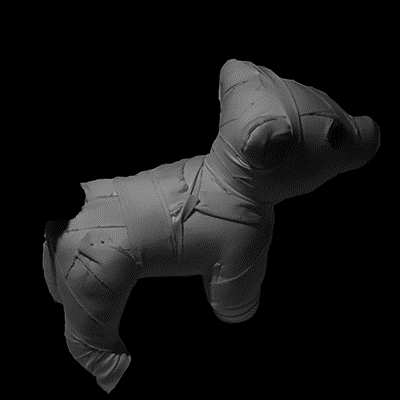
\includegraphics[width = \textwidth]{../dog-png/dog4.png}
  \end{subfigure} 
   \begin{subfigure}[h]{0.3\textwidth}
    \centering
    
\includegraphics[width = \textwidth]{../dog-png/mask.png}
  \end{subfigure} 
%   \begin{subfigure}[h]{0.3\textwidth}
%    \centering
%    \includegraphics[width = \textwidth]{../dog-png/normals.png}
%  \end{subfigure}
  
  \begin{subfigure}[h]{0.3\textwidth}
    \centering
    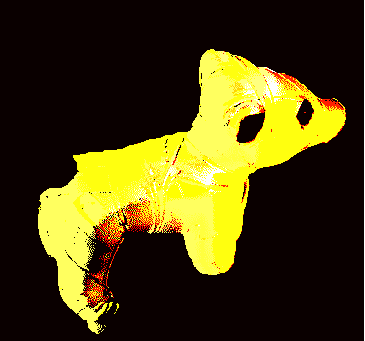
\includegraphics[width = \textwidth]{../dog-png/albedo.png}
  \end{subfigure} 
  \begin{subfigure}[h]{0.02\linewidth}
    \centering
    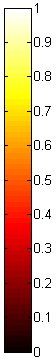
\includegraphics[width = 7mm, height = 48mm]{../dog-png/colorbar.png}
  \end{subfigure} 
    \begin{subfigure}[h]{0.5\textwidth}
    \centering
    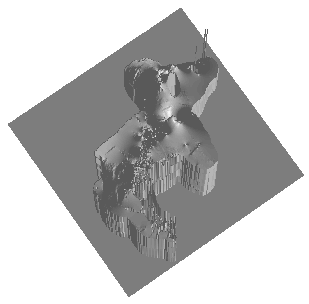
\includegraphics[width = \textwidth]{../dog-png/depthMap.png}
  \end{subfigure} 
   
  \caption{\textbf{Dog-png} dataset. Images shown in order are 4 original images, mask image, \emph{quiver-plot} of surface normals, albedo map and the reconstructed depth.}
  \label{fig6}
  \end{figure}
\end{document}